\documentclass[a4paper, 11pt, onecolumn]{article}
\usepackage[left=2cm, top=3cm, text={17cm, 24cm}]{geometry}
\usepackage{amsmath, amsthm, amssymb}
\usepackage[hidelinks]{hyperref}
\usepackage[utf8]{inputenc}
\usepackage{times}
\usepackage{multirow}
\usepackage[czech]{babel}
\usepackage{graphicx}
\usepackage{float}


\title{ITU\,--\,Štyri v rade} 
\author{Dušan Slúka \\ \href{mailto:xsluka00@fit.vutbr.cz}{xsluka00@fit.vutbr.cz}}
\date{}


\begin{document}
\maketitle

\section*{Výber témy :}
Stránky ktoré používam na hru štyri v rade sú zastarané a ponúkajú minimálnu funkcionalitu.
Štyri v rade (Connect Four) je hra, v ktorej hráči vyberajú farbu a potom striedavo umiestňujú farebné 
žetóny do šesťradového, sedemstĺpcového vertikálne zaveseného hracieho poľa. 


\section*{Zdôvodnenie témy :} 
  Hra má veľkú hráčsku zákľadňu. Pre hráčov je ťažké nájsť modernú verziu medzi aktuálnymi zdrojmy. Stránok ktoré
ponúkajú túto hru je mnoho, no kvalita uživateľského rozhrania je zanedbaná. To isté sa týka funkcionality a variácií.

\section*{Kroky pre zlepšenie :} 
Zameriam sa na moderné a funkčné užívateľské prostredie s možnosťou prispôsobenia prvkov. 
Vytvorím čiastočné úspechy, ktoré by hru urobili zaujímavejšou. 
Vylepším nastavenia hry a ponúknem rôzne varianty, ako napríklad: PopOut, Pop 10, Five-in-a-Row.
\section*{Príklady ktoré ma priviedli k zlepšeniu uživateľského prostredia :} 
\begin{itemize}
  \item https://boardgames.io/en/connect4/gameEnd
  \item https://www.cbc.ca/kids/games/all/connect-4
  \item https://www.mathsisfun.com/games/connect4.html
\end{itemize}
\newpage
\section{Dotazník}
\subsection{Otázky}
\begin{enumerate}
    \item Ako často hráte hru štyri v rade?
    \item Na akom zariadení by ste najradšej hrali štyri v rade?
    \item Čo vás na hre štyri v rade najviac baví?
    \item Čo vás pri hraní štyri v rade na súčasných platformách frustrovalo?
    \item Máte záujem o možnosti hry pre viacerých hráčov na jednom zariadení?
    \item Mali by vás zaujímať pokročilé funkcie ako analýza hry alebo štatistiky hráčov?
    \item Ako dôležité je pre osobné prispôsobenie hráčskeho rozhrania?
    \item Ako dôležitá je pre vás grafika a vizuálne efekty pri hraní?
    \item Čo by vás motivovalo hrať štyri v rade častejšie?
    \item Aké sú vaše obľúbené alternatívy k hre štyri v rade?
    \item Aké ďalšie funkcie alebo vylepšenia by ste radi videli na novej platforme pre hru štyri v rade?
\end{enumerate}
\subsection{Respondenti}
Dušan Slúka:
Dotazník bol poskytnutý piaťim osobám.
S dvomi z nich som sa stretol a ich odpovede aj prediskutoval a vypítal si odôvodnenie.
Sú to hráči ktorí sa vracajú k hre aspoň dva krát do mesiaca. Čo je aj moja skupina zamerania. 

\section{Poznatky z odpovedí}

Na základe dotazníka sme získali nasledovné poznatky:
Jakub Majer:
Ivan Mahút:
Dušan Slúka:
\begin{itemize}
    \item U väčšiny respondentov ,hra štyri v rade nie je ich každodennou aktivitou.
    \item Existuje rovnaký záujem o hranie na smartfóne, počítači či naživo.
    \item Hráči oceňujú jednoduchosť a logickú výzvu hry.
    \item Najväčšou frustráciou hráčov je slabé užívateľské rozhranie a nedostatok funkcií.
    \item Všetci respondenti by mali záujem o možnosť hry pre viacerých hráčov na jednom zariadení.
    \item Respondenti majú zmiešaný názor na potrebu pokročilých funkcií.
    \item Osobné prispôsobenie hráčskeho rozhrania nie je pre respondentom dôležité.
    \item Grafika a vizuálne efekty sú pre väčšinu respondentov dôležité.
    \item Nové herné režimy a možnosť súťažiť s priateľmi by motivovalo hráčov k častejšiemu hraniu.
    \item Respondenti preferujú rôzne alternatívy k hre štyri v rade.
\end{itemize}

\section{Analýza odpovedí}

\subsection{Potreby užívateľov}
Na základe získaných odpovedí je možné identifikovať nasledujúce potreby užívateľov:
Jakub Majer:
Ivan Mahút:
Dušan Slúka:
\begin{itemize}
    \item Zlepšenie užívateľského rozhrania.
    \item Pridanie nových funkcií.
    \item Zlepšenie grafiky a vizuálnych efektov.
    \item Pridanie odmien a funkcí na zvýšenie frekvencie hrania.
    \item Možnosť hrať s priateľmi.
\end{itemize}

\subsection{Kľúčové problémy}
Jakub Majer:
Ivan Mahút:
Dušan Slúka:
\begin{itemize}
    \item Slabé užívateľské rozhranie.
    \item Nedostatok funkcií a herných režimov.
    \item Hra nedisponuje funkciami, ktoré by hráčov motivovali k návratu.
\end{itemize}

Jakub Majer:
Ivan Mahút:
Dušan Slúka:
\section{Existujúca aplikácia: \href{https://boardgames.io/en/connect4/gameEnd}{boardgames.io/connect4}}

Táto online verzia hry Štyri v rade na platforme boardgames.io ponúka veľmi jednoduchý a 
priamočiary prístup a dizajn.

\subsection{Prednosti:}
\begin{itemize}
    \item \textbf{Jednoduchosť}: Hra je intuitívna a ľahko prístupná pre nových hráčov.
    \item \textbf{Priamočiarosť}: K hraniu hry sa dostanem po kliknutí jedného tlačidla. 
    \item \textbf{Responzívnosť}: Aplikácia je optimalizovaná pre rôzne zariadenia, vrátane mobilných telefónov a tabletov.
\end{itemize}

\subsection{Nedostatky:}
\begin{itemize}
    \item \textbf{Obmedzená funkcionalita}: Aplikácia neponúka žiadne rozšírené nastavenia či funkcionalitu.
    \item \textbf{Nedostatok prispôsobenia}: Hráči nemajú možnosť upravovať a prispôsobovať herné rozhranie podľa svojich preferencií.
    \item \textbf{Grafický aspekt}: Absencia grafických nápovied a animácií pre príťažlivejšie prostredie.
    \item \textbf{Varianty}: Jedinou variantou je hra štyri v rade čo obmedzuje návrat k platforme.
\end{itemize}

\subsection{Poznatky získané pre našu verziu aplikácie}

Na základe analýzy existujúcej aplikácie plánujeme vytvoriť novú verziu hry 
Štyri v rade, ktorá bude zahŕňať prednosti súčasnej aplikácie, ale zároveň 
bude riešiť jej nedostatky. Naším hlavným cieľom je ponúknuť hráčom moderné, 
prispôsobiteľné a funkčné užívateľské rozhranie s pokročilými funkciami 
a možnosťami.

\section{Rozdelenie práce a varianta}

Rozhodli sme sa pre variantu dva. Každý člen vypracuje časti aplikácie.
Dušan Slúka: Hlavné menu,Obrazovka hry 4-vrade,Modálne okno pre výhru, Modely pre tieto scény, Pislúchajúca časť backendu.\\
Jakub Majer:
Ivan Mahút:
\section{Maketa}
Jakub Majer:
Ivan Mahút:
Dušan Slúka:
\subsection{Hlavné menu:}
\begin{figure}[H]
  \centering
  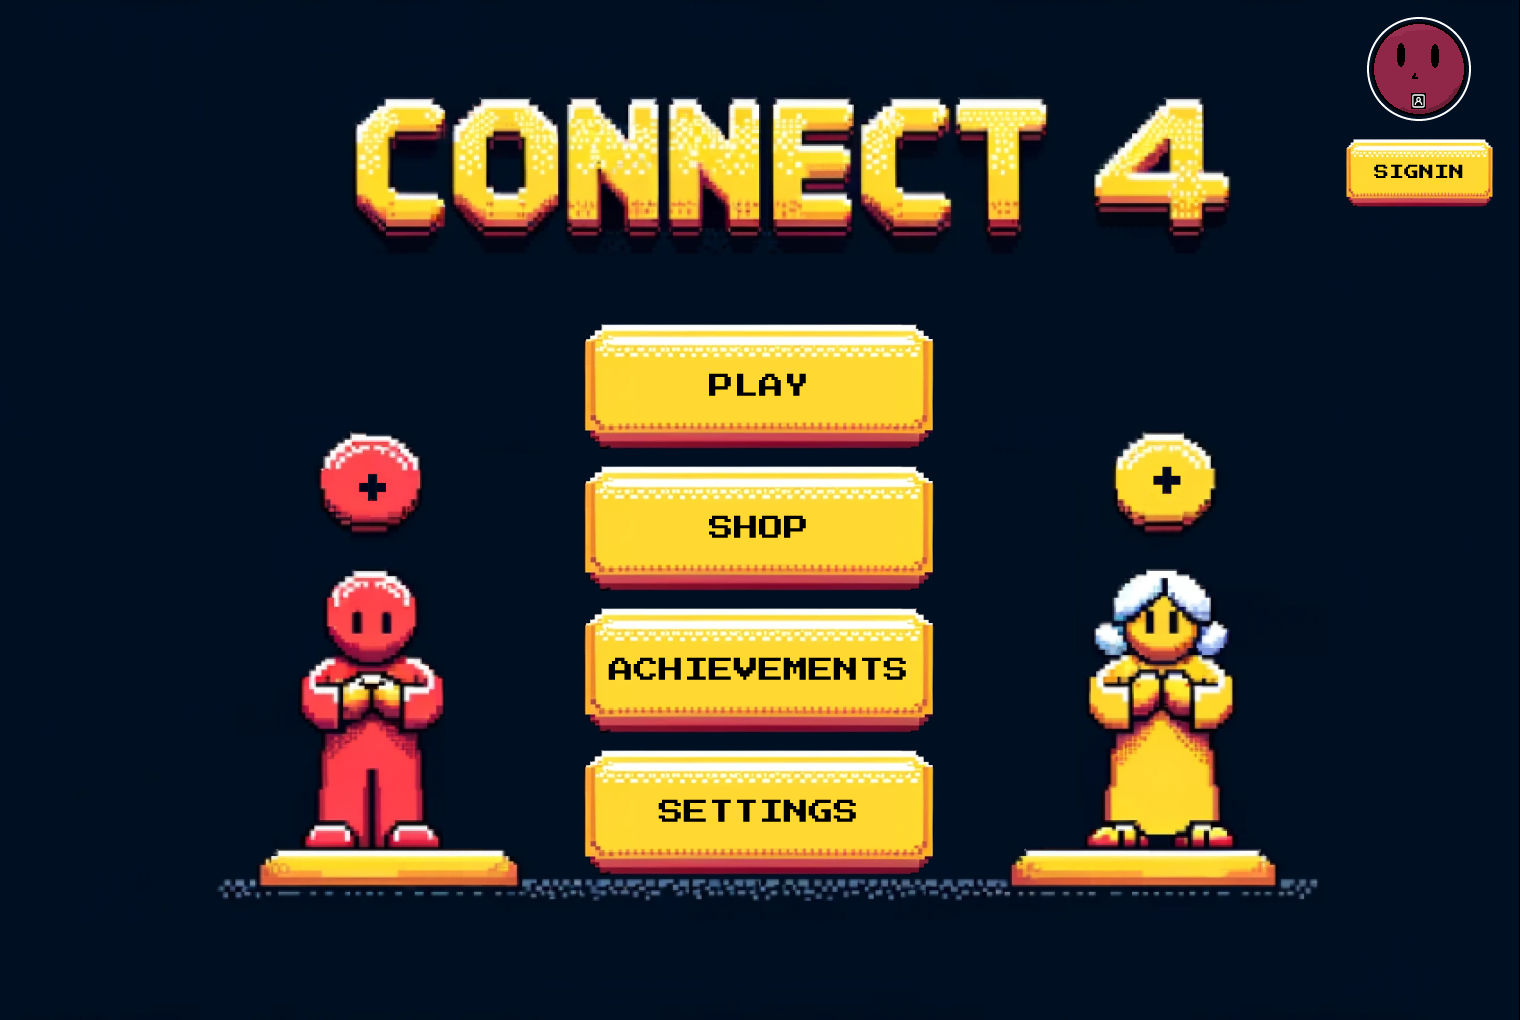
\includegraphics[width=0.8\textwidth]{Menu.png}
  \caption{ Menu hry.}
  \label{fig:menu_label}
\end{figure}

\subsection{Hracia plocha:}
\begin{figure}[H]
  \centering
  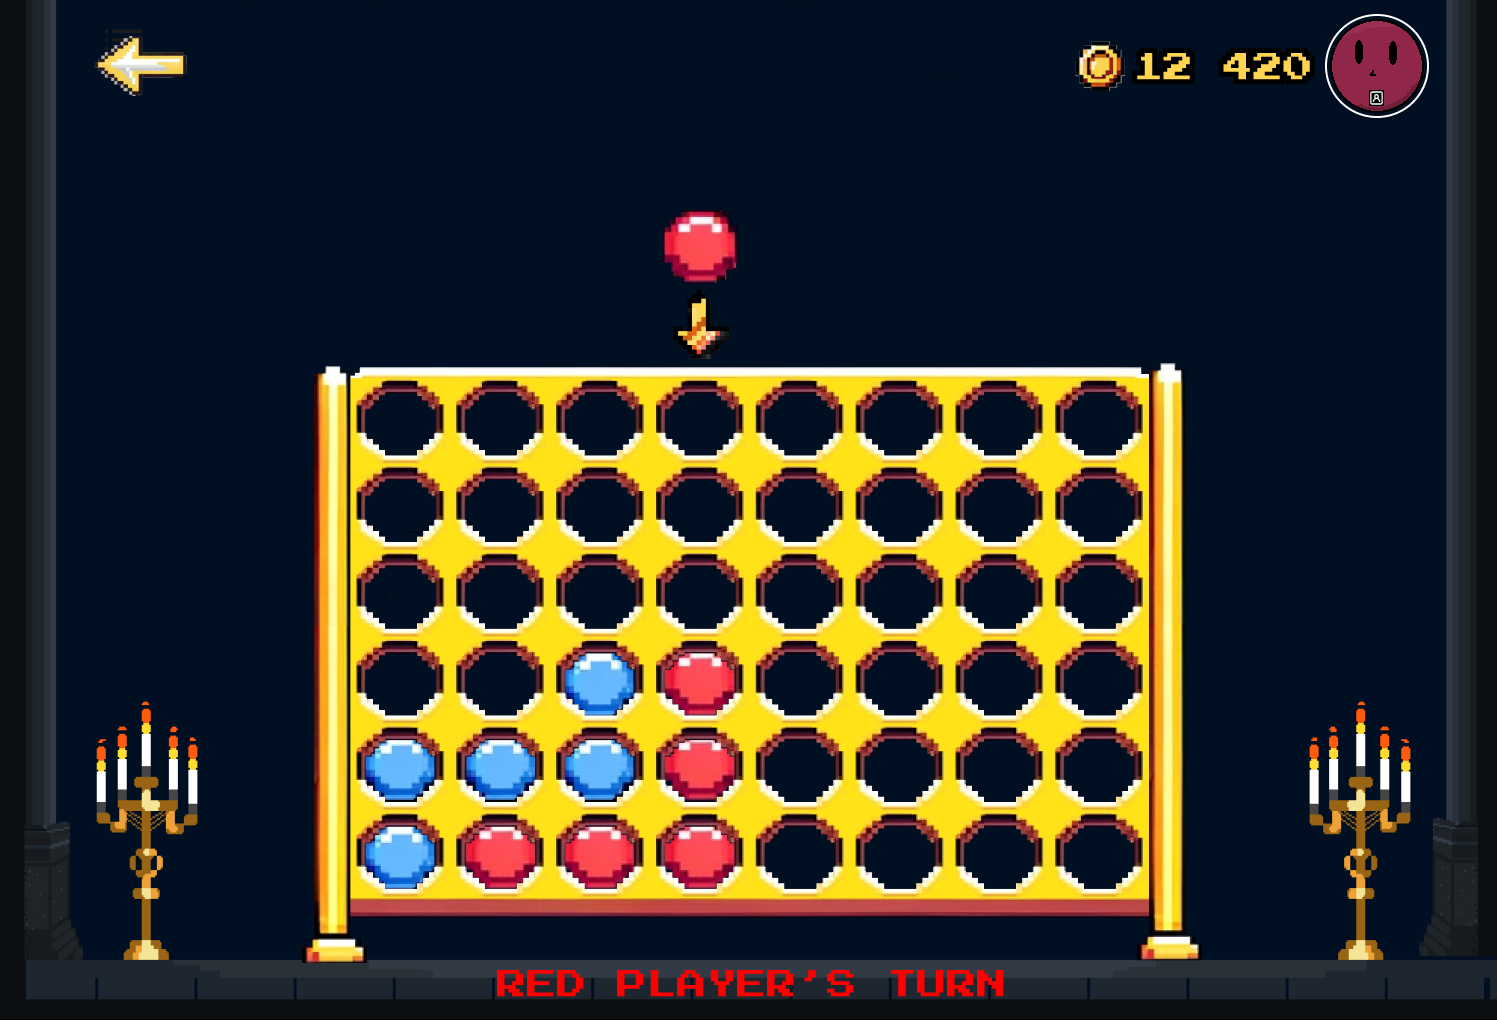
\includegraphics[width=0.8\textwidth]{Plocha.png}
  \caption{ Hracia plocha pre štandardnú verziu.}
  \label{fig:štandard_label}
\end{figure}

\subsection{Modálne okno sumarizácie hry:}
\begin{figure}[H]
  \centering
  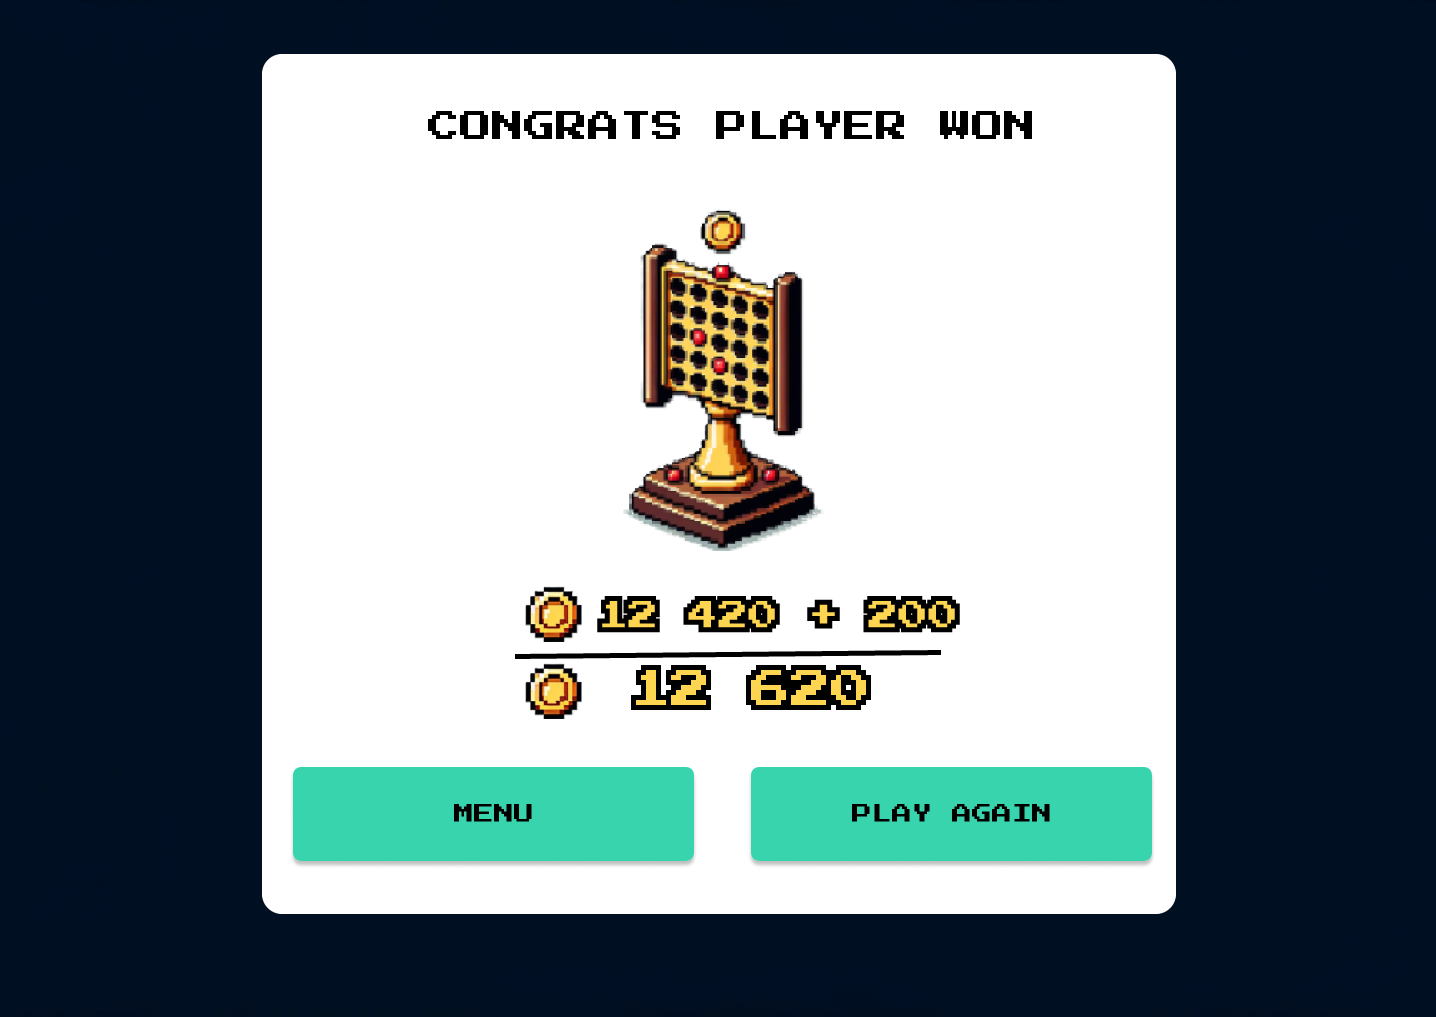
\includegraphics[width=0.8\textwidth]{Vyhra.png}
  \caption{ Sumár po odohraní partie.}
  \label{fig:sumár_label}
\end{figure}

\subsection{Riešenie potrieb užívateľov}
Jakub Majer:
Ivan Mahút:
Dušan Slúka:
\begin{enumerate}
    \item \textbf{Zlepšenie užívateľského rozhrania:} Makety znázorňujú, že sme aktualizovali užívateľské rozhranie hry "Connect 4" s cieľom zvýšiť jeho intuitívnosť a vizuálnu atraktivitu. Rozloženie menu a možnosti sú jasne definované a prístupné.
    \item \textbf{Zlepšenie grafiky a vizuálnych efektov:} Namiesto nudných a už zaužívaných prvkou sme sa rozhodli pre viacej atraktívnejšiu formu uživaťeľského prostredia ktorou je "pixelart". Táto voľba nám dovolila si vo vlastnej réžií navrhnúť a nakresliť väčšinu prvkov čo vyustilo k estetickému dizajnu.
    \item \textbf{Možnosť hrať s priateľmi:} Hra je navrhnutá tak aby vedeli dvaja hráči hrať na jednom zariadení a intuitívne zistili v akom štádiu hra je a čo robiť.
\end{enumerate}

\subsection{Kľúčové problémy a riešenia}
Jakub Majer:
Ivan Mahút:
Dušan Slúka:
\begin{itemize}
    \item \textbf{Slabé užívateľské rozhranie:} Nové užívateľské rozhranie je jasné a intuitívne, zamerané na zlepšenie skúsenosti hráča.
    \item \textbf{Nedostatok herných režimov:} V aktuálnej verzí sú dostupné dva herné režimy pre ktoré sú vytvorené pre dlh3ie udržanie a väčšiu návratnosť hráča.
\end{itemize}

\end{document}

\end{document}